\documentclass[11pt,notitlepage]{article}
\usepackage{graphicx}
\usepackage{cite}
\usepackage{braket}
\usepackage{amssymb}
\setcounter{tocdepth}{3}
\usepackage{graphicx}
\usepackage{algorithm}
\usepackage{algorithmic}
\usepackage{multirow}
\usepackage{extarrows}
\usepackage{epstopdf}
\usepackage{url}
\usepackage{multicol}
\usepackage{amssymb}
\usepackage{booktabs}
\usepackage{array}
\usepackage{calc}
\usepackage{subfigure}
\usepackage{url}
\usepackage[toc,page,title,titletoc,header]{appendix}
\usepackage{mathrsfs}
\usepackage{braket}
\usepackage{bm}
\usepackage{color}
\usepackage{hyperref}


% font

\usepackage{palatino} % Palatino font
%\usepackage{helvet} % Helvetica font
\renewcommand*\familydefault{\sfdefault} % Use the sans serif version of the font
\usepackage[T1]{fontenc}
\linespread{1.05}

% margin
\usepackage[top=0.5in,bottom=0.5in,left=0.5in,right=0.5in]{geometry} 


\author{Benyou Wang \\ \href{mailto:waby@tju.edu.cn}{waby@tju.edu.cn}
% \and jingfei li \\ ljf@tju.edu.cn
}
\title{A Study of Infererence Term in the Real Vector Space}
\begin{document}
\tableofcontents
\maketitle

\abstract{ Recenty, Quantum theory(QT) have been applied to many fields outside physics, e.g., Information Retrieval(IR). \emph{Phrase} with a complex-number reprentation, one of the key property,  has been ignored in IR for the sake of computational feasibility. This paper tries to explore the nature of interfence term in real vector space, which indictas that the interference effect can hardly be observed and the judgement discrepency may derive from the multiple collapse instead of single}

\section{the Double-Slit Experiment}

In the Young's Double-Slit interference experiment, some scientists demostrate that the photons (and other atomic-scale entities such as electrons) can display characteristics of both classically defined waves and particles. A wave of the light is considerd into two separate waves that later combine into a single wave. Difference in the path lengths of both waves results in a phase shift, creating an interference pattern which contains many fringes of bright and shade. 

When the emitter was restricted to shoot only one photon within a short time, we still get the superposed images of fringes. Based on the fundamentally probabilistic nature of quantum mechanical phenomena, the Copenhagen School propose a new explanation that the photon may pass through the two slit simultaneously and the photon may interference with the other one of itseltf which result in the stripy phenomenon.


\begin{figure}[htbp]
\centering
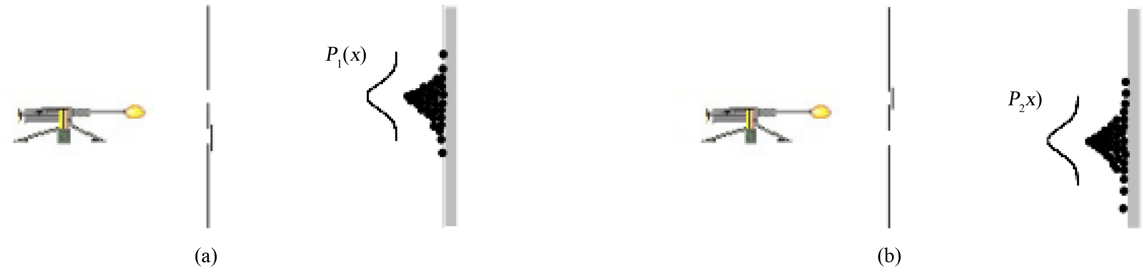
\includegraphics[width = 12 cm]{graph/wave.pdf}
\caption{Two examples of the images}
\label{fig:quantum}
\end{figure}


We define the quantum state of a system as a wave function. in the Young's Double-Slit interference experiment, the wave function is defined as $\psi(x)$, where $x$ is the positon on the screen and $\psi(x)$ denotes the probablity amplitude (a complex number) that the photon exists in specific position $x$. The square modulus of the wave function $\left|\psi (x,t)\right|^{2}={\psi (x,t)}^{*}\psi (x,t)=\rho (x,t)$, which is a positive real number,
is interpreted as the probability density that the particle is at x.

Due to the interference effect, the images on the screen with two waves is not the classical superposition of the two wave function(which means  $\psi_1(x)$+ $\psi_2(x)$ ), which seems to be vollidated with our common sense. Namely, we can only oberserve the intensity of light by our naked eye, the hidden phase of a single photon in the micro wolrd cannot be perceived by human. Due to the consideration of the phase, the intensity of light on the specific postion $x$ will enhance while the photons from the another slit have the similiar phases with the first one, and fade while the opposite phases.   
\begin{equation}
\rho(x)=\rho_1(x)+\rho_2(x)+2\sqrt{\rho_1(x)\rho_2(x)}cos\theta \neq \rho_1(x)+\rho_2(x)
\label{eq:wave_function}
\end{equation}
While $\theta$ is the phase difference at position $x$ between two waves. In the unknown confition, in which the observers can not confirm which slit does the photon pass through, the interference effect will works.

\section{Interference Effect in Cognition}

Recently, Quantum Theory have been introducing to many fields outside phisics, e.g., cognitive sicence. It may be inherent that the concept of {\em{probability}} is both objective and subjective in cogintive science. When responsing to the a dichotomous attitude of a question, the probability of the our attitude have two discrete value, e.g. Yes or No. These two values is analogous to the continuous position on the screen in the double-slit experiment.

A person's belief about the subjective attitude on the decision or question is presented by a state vector in a multidimensional Hilbert space, the belief state is described as a wave function which can tells us the probatilistic distribution of different possibility (different posion in the double-slit experiment or the different attitudes in the prisoner dilemma). 

\begin{equation}
\ket{S}=\alpha \ket{0}+ \beta \ket{1}
\label{eq:belief_state}
\end{equation}

while $\ket{0}$ and $\ket{1}$ denotes the diffierent anwsers to the question, $\alpha$ and $\beta$ denotes the probability amplitude of such event.  $\alpha$ and $\beta$ are complex numbers and their squared values is the corresponding probability $p(0)=\alpha^2+\beta^2$. Apparently it will satisfy the probabilty normalization condition $\alpha^2 +\beta^2 =1$.

Von Neumann postulates that the measurement will lead to a collapse of the current vector state. This postulation inspire us to model the dynamic nature of decision-making process over time. Different orders of the measurement will constitute different context for human's response to the outside. This context-sensitive processes provide a strong ability to explain some non-classical phenomenon which seems hardly interpreted in a classic framework.

Another typical experiment called "prisoner dilemma" provides a apparent violation of the classical theory of probability. When the participants have known that the another have defected, this information will change his behavior in one pattern (means a wave function or a probability distribution of his final choice). When not defected, there will be another pattern. But if the person do not know the decision of the another, the behavior pattern is not simplely the classical superpostion of the premier two patterns. Analogy to the double-slit experiment, maybe we can know the final probability (the intensity of the light) of the each separate actions in the certain condition, but we can not know the hidden phase of each one and the complex superposition of the two certain condition due be the ignoration of the hidden phase.

We follow the Von Neumann's postulation of collapse, in the known condition, we have
\begin{equation}
\begin{split}
p'(d)=&\Vert\Pi_{d}\Pi_{od}S\Vert^2+\Vert\Pi_{d}\Pi_{oc}S\Vert^2 \\
=&\vert \braket{S_{od}|S}|^2*|\braket{S_d|S_{od}} \vert^2 +\vert \braket{S_{oc}|S}|^2*|\braket{S_d|S_{oc}} \vert^2
\end{split}
\label{eq:known}
\end{equation}
while in the unknown condition, we have
\begin{equation}
\begin{split}
p(d)=&\vert \braket{S_d|S}\vert ^2=\Vert\Pi_dS \Vert^2 \\
=&(\braket{S_{od}|S} *\braket{S_d|S_{od}} +\braket{S_{oc}|S}* \braket{S_d|S_{oc}})^2 \\
=&|\braket{S_{od}|S}|^2*|\braket{S_d|S_{od}}|^2  +|\braket{S_{oc}|S}|^2*|\braket{S_d|S_{oc}}|^2 \\
&+\mathbf{2\vert \braket{S_{od}|S} \braket{S_d|S_{od}} \braket{S_{oc}|S} \braket{S_d|S_{oc}} \vert cos(}\theta)
\end{split}
\label{eq:unknown}
\end{equation}
The additional term in the forth line of Equation \ref{eq:unknown} is called "interference term", and the $\theta$ denotes the phase difference.

\section{interference terms in the real vetor space}

In the double-slit experiment, we cannot oberserve any interference effect if the photons have the same phase. How about the process of belief-adjustment collapse in the real vector space?

\begin{figure}[!htb]
\centering
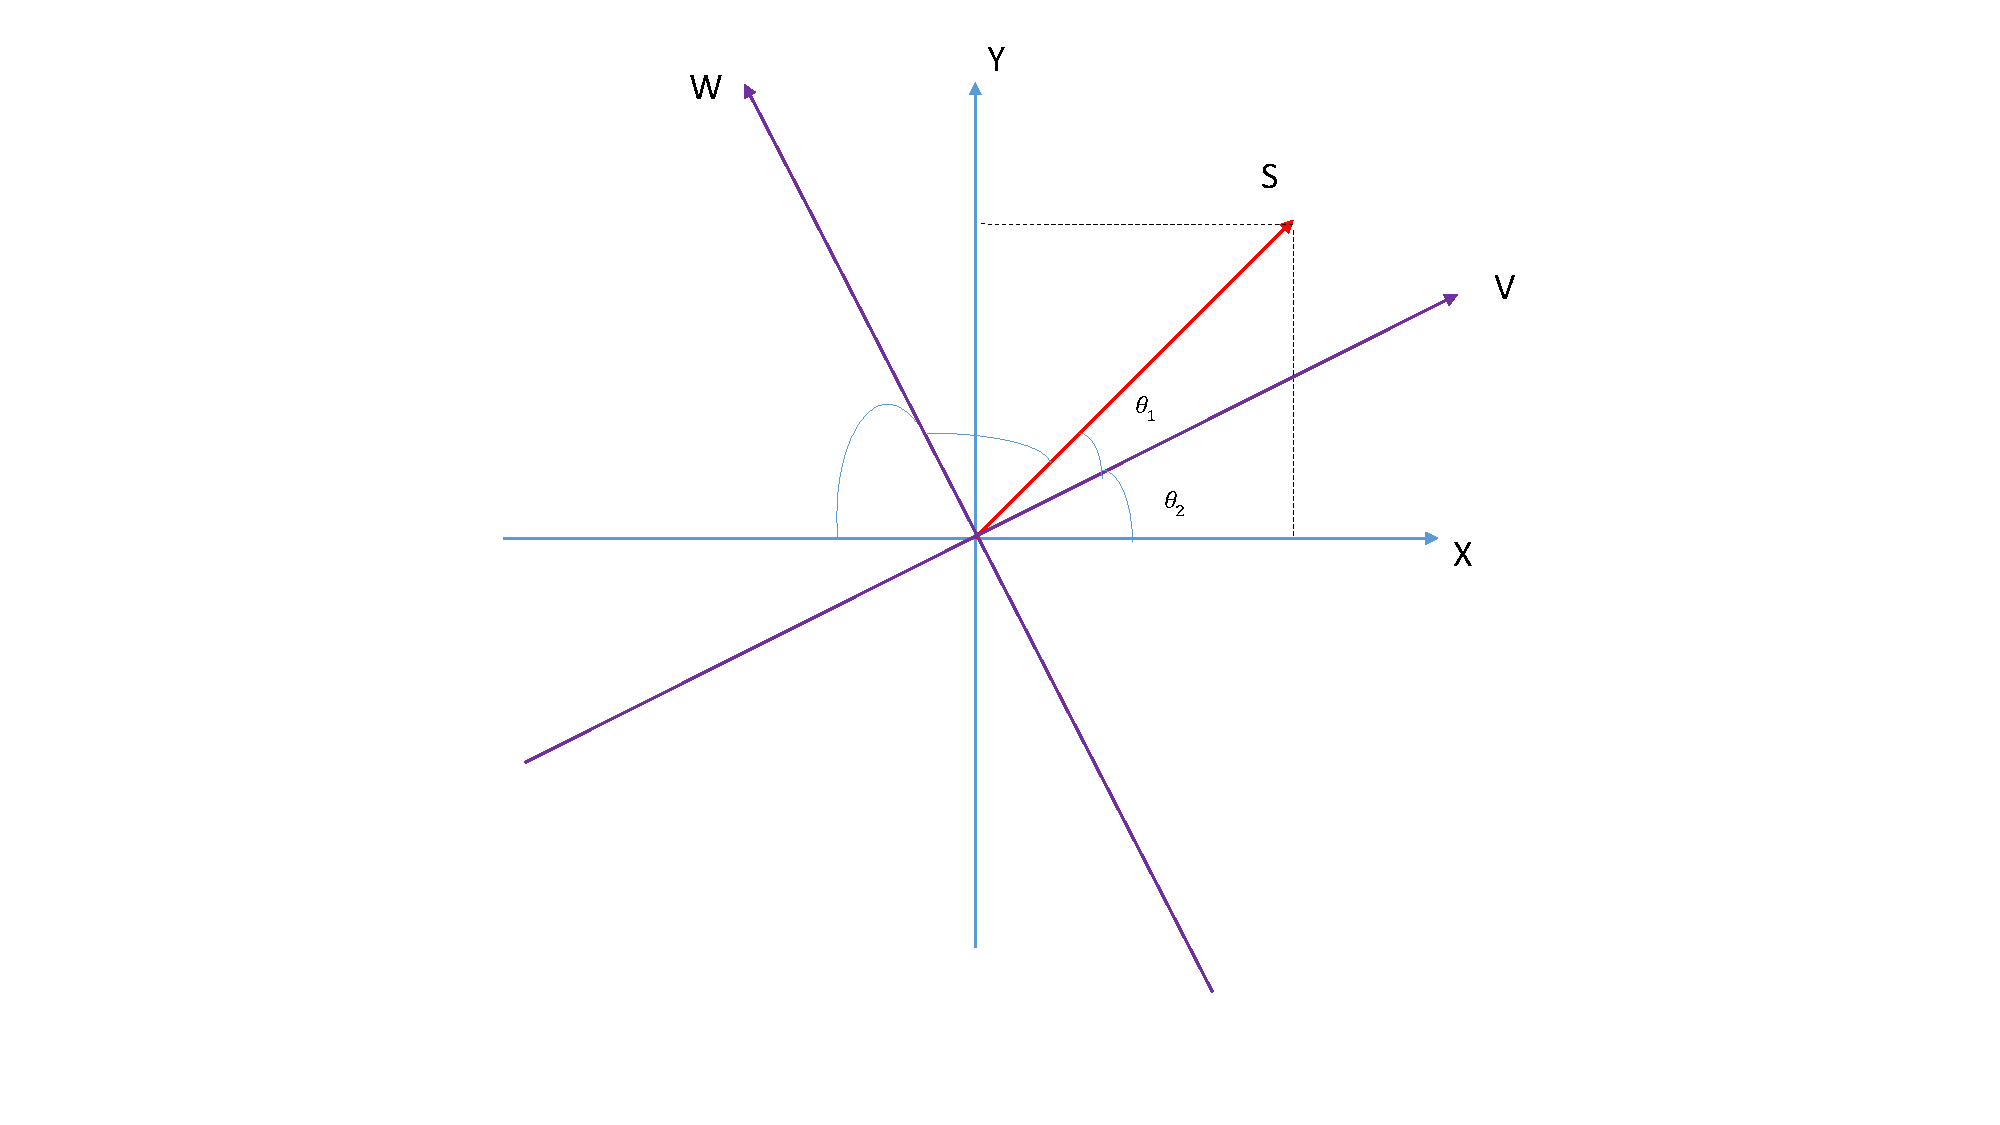
\includegraphics[width = 12 cm]{graph/projection.pdf}
\caption{The projection of the interference in the real vector space}
\label{fig:projection}
\end{figure}

Due to the lack of intuitive meaning of the complex field in some subjects like Information Retrieval (IR), reserachers usually adopt the real field of the probability amplitudes for the sake of computational feasibility. In the real vector space, these numbers are have the imaginary part of zero. Consequently, the phase difference at any position between two waves will keep zero, $\theta=0$ and $cos(\theta)=1$. The Equation \ref{eq:unknown} can be rewritten as follow in the real vector space:
\begin{equation}
\begin{split}
p(d)=&\vert \braket{X|S}\vert ^2 \\
=&(\braket{W|S} *\braket{X|W} +\braket{V|S}* \braket{X|V})^2 \\
=&|\braket{W|S}|^2*|\braket{X|W}|^2  +|\braket{V|S}|^2*|\braket{X|V}|^2 \\
&+\mathbf{2\vert \braket{W|S} \braket{X|W} \braket{V|S} \braket{X|V} \vert }
\end{split}
\label{eq:unknown_real}
\end{equation}

With the change of the angel between the two basis, we get the probabilities of the first path, the second path (in analogy to two slits) and the both. 
\begin{figure}[!htb]
\centering
\includegraphics[width = 12 cm]{graph/interference.eps}
\caption{the probabilities of different condition and the interference term}
\label{fig:interference_real}
\end{figure}
As showed in the Figure \ref{fig:interference_real}, the interference term is the difference between the probability of one-time measurement and the additive probabilities of two-times measuments which is labeled with the black line.
In the perspective of he projection, we get the interference term as the following format

\begin{equation}
\begin{split}
interferenceTerm=&2\vert \braket{W|S} \braket{X|W} \braket{V|S} \braket{X|V} \vert \\
=&2cos(\theta_1)cos(\theta_2)sin(\theta_1)cos(\theta_2) \\
=&\frac{1}{2}sin(2\theta_1)sin(2\theta_2)
\end{split}
\label{eq:interference_term_in_projection}
\end{equation}
$\theta_1$ is the orginal angle bewteen the belief state with the one arbitrary basis which is dependent with the final measurement basis. while $\theta_2$ is the angle between the two basis which are from the two pair of orthogonal basis, respectively. $\theta_1$ and $\theta_2$ satisfiy that $\vert \theta_1 -\theta_2 \vert = angle(S,X)$ or $\vert \theta_1+\theta_2=angle(S,X)$. angle(S,X) is a a priori parameter which keeps unchanged in a specific condition. $\theta_1$ and $\theta_2$ are only decided by the relation between the two pairs of the orthogonal basis. Technically speaking, this relation may be driven by the concept of {\em{incompatibility}} in Quantum Theoty. If two measuments are compatible, the interference term will turn to zero(In the Figure \ref{fig:interference_real}, the horizontal ordinate is be divided by $\frac{\pi}{2}$ with no remainder)
% \subsection{Beijing} Beijing is the capital of China
% \subsubsection{Dongcheng district}
% \paragraph{Tian'anmen Square} is in the center of Beijing
% \subparagraph{Chairman Mao} is in the center of Tian'anmen Square
% \subsection{Guangzhou}
% \paragraph{Sun Yat-sen University} is the best university of in Guangzhou
\section{conclution}
Although the interference effects still exist in the real vector space. Due to lack of the imaginary part, the interference effect will lose much representive power to discribe the state of the system. The deep reason of the interfernce effect is not the hidden phase like the double-slit experiment, but the dynamic adjustment of the belief state based on the postulation of the collapse. 

\end{document}
